
\section {物料建模}
        .
        \begin{center}
            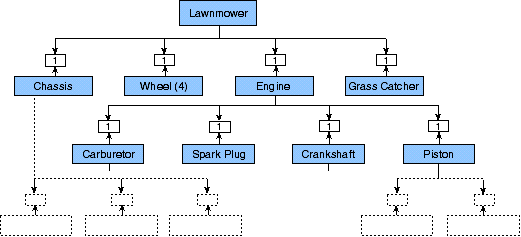
\includegraphics[scale=0.6] {bom1.png}
        \end{center}

          物料清单(Bill of Materials,简称BOM)是描述企业产品组成的技术文件。在加工资本式行业,它表明了产品的总装件、分装件、组件、部件、零件、直到原材料之间的结构关系,以及所需的数量。在化工、制药和食品行业产品组成则对主要原料、中间体、辅助材料及其配方和所需数量的说明。物料清单是将用图表示的产品组成改用数据表格的形式表示出来,它是计算MRP过程中的重要控制文件。

\subsection {物料清单的基本资料}

    构成父项装配件的所有子装配件、中间件、零件及原材料的清单,其中包括装配所需的 各子项的数量。物料清单和主生产计划一起作用,来安排仓库的发料、车间的生产和待采购件的种类和数量。可以用多种方法描述物料清单,如单层法、缩进法、 模块法、暂停法、矩阵法以及成本法等等。在某些工业领域,可能称为“配方”、“要素表”或其他名称。

    物料清单是一个制造企业的核心文件,各个部门的活动都要用到物料清单。生产部门要根据物料清单来生产产品,仓库要根据物料清单进行发料,财会部门要根据物料清单来计算成本,销售和订单录入部门要通过物料清单确定客户定制产品的构形,维修服务部门要通过物料清单了解需要什么备件,质量控制部门要根据物料清单保证产品正确地生产,计划部门要根据物料清单来计划物料和能力的需求,等等。

    物料清单根据使用目的或特点不同,有多种表现了形式,例如单级BOM,多极BOM、百分比式的计划用BOM、模式化BOM、制造BOM和虚拟BOM等。

    \begin{itemize}
        \item  狭义上的BOM(Bill of Materials)通常称为“物料清单”,就是产品结构(Product Structure)。仅仅表述的是对物料物理结构按照一定的划分规则进行简单的分解,描述了物料的物理组成。一般按照功能进行层次的划分和描述。
        \item  广义上的BOM是产品结构和工艺流程的结合体,二者不可分割。离开工艺流程谈产品结构,没有现实意义。要客观科学的通过BOM来描述某一制造业产品,必须从制造工艺入手,才能准确描述和体现产品的结构。
    \end{itemize}

    物料清单是说明一个最终产品是由哪些零部件、原材料所构成的,这些零部件的时间、数量上的相互关系是什么。这种产品结构反映在时间结构上,则以产品的应完工日期为起点倒排计划,可相应地求出各个零部件最晚应该开始加工时间或采购订单发出时间,当一个最终产品的生产任务确定以后,各零部件的订单下达日期仍有先有后。即在保证配套日期的原则下,生产周期较长的物料先下订单,生产周期较短的物料后下订单,这样就可以做到在需用的时候,所有物料都能配套备齐;不到需用的时候不过早投料,从而达到减少库存量和减少占用资金的目的。

\subsection {物料清单类型}

    \subsubsection {标准物料清单:标准物料的物料清单。}

    标准物料指包含在物料清单上除计划物料、选项类或模型之外的物料,如采购件、自制件、委外件等。标准物料清单是最常用的清单类型,其列有法定的子件、每个子件的需求数量、在制品控制信息、物料计划等功能。

    \subsubsection {计划物料清单:计划物料的物料清单。}

    代表一个产品系列的物料类型,其物料清单中包含子件物料和子件计划百分比。可以使用计划清单来帮助执行主计划和(或)物料需求计划。

    \subsubsection {模型物料清单:模型物料的物料清单。}

    模型物料是指在订购该物料时,其物料清单会列出可选用的选项和选项类的物料。模型物料清单列出了模型所具有的选项类、选项和标准物料,可以在销售系统中按客户要求订购不同的产品配置。模型清单可以是按订单装配(ATO:Assemble-to-order)或按订单挑库(PTO:Pick-to-order)类型的,ATO与PTO模型的区别在于,ATO需选配后下达生产订单组装完成再出货,PTO则按选配子件直接出货。

    \subsubsection {选项类物料清单:包含一系列相关选项的选项类物料的物料清单。}

    选项类就是物料清单上对可选子件的一个分类。选项类作为一个物料,成为模型物料清单中的一层。

    虚拟件:虚拟件是一个无库存的装配件,它可以将其母件所需物料组合在一起,产生一个子装配件。MPS/MRP系统可以通过虚拟件直接展开到该虚拟件的子件,就好似这些子件直接连在该虚拟件的母件上。 应用:作为共用件,让物料清单较容易维护,使产品结构清晰,并减少工作量。

    公用物料清单:任何具有同一清单类型的两个物料均可以共享公用物料清单。如果两个不同的物料共享同一清单,那么只需定义好一个物料的清单,可供另一物料公用,但这两个物料应该具有相同的BOM类型。定义新的母件的物料清单时,可将另一母件作为公用物料清单来引用,而不需在物料清单中输入任何信息,节省输入时间并方便维护。

\subsection {物料清单的基本功能}

    物料清单是企业所有核心业务都要用到的共享管理文件,关键词是“共享”,就是说,它对任何业务都是重要的,不是某一种业务所独占的文件。但要求物料清单全面细致、使用最频的是计划与控制部门。

    物料清单是产品结构的技术性描述文件,它不仅列出最终产品的所有构成项目,同时还表明这些项目之间的结构关系, 即从原材料到零件、组件,直到最终产品的层次隶属关系,以及它们之间的数量关系。物料清单是制造企业的核心文件,各个不同的部门和系统都要用到物料清单,从物料清单中获取特定的数据,因此物料清单是联系与沟通企业各项业务的纽带,企业各个业务部门都要依据统一的物料清单进行工作:

    \begin{itemize}
        \item  设计部门是物料清单的设计者,也是物料清单的使用者, 需要从物料清单中获取所有零件的信息以及相互间的结构信息;
        \item  工艺部门根据物料清单建立各零件的制造工艺和装配件的装配工艺,以及加工制造过程中应使用的工具、模具等;
        \item  生产部门根据物料清单来生产产品;
        \item  库房根据物料清单进行发料,是仓库部门向生产工位配套发料的依据;
        \item  财务部门根据物料清单中每个自制件或外购件的成本来确定最终产品的成本;
        \item  销售和订单录入部门要通过物料清单确定客户定制产品的构形,它确定配置产品需用的可选伟计算累计提前期、是销售部门洽谈客户定单的依据;
        \item  质量控制部门要根据物料清单保证产品的正确生产;
        \item 计划部门要根据物料清单来计划物料和能力的需求,物料清单是按照实际的生产装配顺序编制的,是计划部门编制生产计划和采购计划的依据;
        \item  维修部门通过物料清单了解最终产品的具体结构,了解需要哪些备件等等。
        \item 是跟踪物流,工序及生产过程、追溯任务来源的依据;
        \item 是供应部门采购和外协的依据;
        \item 是改进产品设计的3化工作(标准化、系列化、通用化)需要参照的重要文件;
        \item 是销售部门投标报价的依据。当遇到一个新产品要报价时,如果新产品同老产品是结构相似、工艺相近,负责报价的部门可以从各个老产品中,摘出相似的相关单层结构,重新“拼凑”成一个结构近似的假想新产品。运用系统的成本累加功能计算出它的成本,作为迅速而比较准确的报价依据。
        \item 如果把工艺装备也包括在物料清单中,就可以同步地生成生产准备计划,并按所加工的零件数量合理分摊消耗工艺装备的“间接”成本。
    \end{itemize}

    可见物料清单对于企业各部门的管理工作有着十分重要的作用; 上述各项业务涉及销售、计划、生产、供应、物料、成本、设计、工艺等部门,物料清单体现了信息集成和共享。对一个制造业企业来讲,实现信息化管理离了物料清单是不能运行的。 物料清单功能的深入研究,对于经营管理中各项功能的优化整合有着十分重要的意义。

    同时,物料清单又是使系统能够识别产品结构。用计算机辅助管理,首先要使系统能够 "读出” 企业制造的产品结构和所有涉及到的物料。为了便于计算机识别,必须把用图表达的产品结构转换成数据报表格式,也就是物料清单。物料清单同产品结构图所说明的内容是一致的。

    我国有一些企业,如大连起重机厂的销售计划科就曾用拼凑单层产品结构的方法形成模拟产品,迅速做出新产品的报价;也有一些企业,如哈尔滨汽车电器厂的财务科在产品结构的基础上,用自底向上累计的方法计算成本。这些例子都发生在20世纪80年代,是国内企业一些部门在没有听说过 MRP 的情况下的管理创新,说明 MRP 这种“产品结构”的思维方法反映了生产客观规律,对任何地域和体制都是适用的,不能简单地把它看成是“舶来品”。只是我国企业的这些管理创新,没有人对它再进行深层次的研究,提升为管理理论。这也反映我围对应用科学的忽视,值得深刻反思。

    正因为物料清单是系统识别产品的依据,说明产品是如何“做出来”的,要为企业众多部门所应用。它的准确度必须要求达到100\%。物料清单是“时间坐标上的产品结构”数据模型的报表形式,说明动态的期量标准,如果模型不准确,运行 MRP 的结果会完全失去意义。

    建立物料清单,从表面上看似乎会给企业的某些部门增加了工作量,但从企业管理整体来看,将减少各个部门在查询、统计、传递和复制报表等方面的大量的工作,要用全局观点来对待物料清单。在 ERP 内部集成系统同 CAD 和 PDM(产品数据管理)系统集成的情况下,可以在设计图纸的基础上,经过适当补充调整,转换成制造用的物料清单,从而减少大量的重复工作。

\subsection {产品是由众多 “单层结构” 组成的}

    物料和由物料组成的 "单层结构” 是产品结构的基本单元。

    任何一个产品都是由若干个 "单层结构” 组成的,单层结构中的上层物料,我们称为 “母件 (parent)”,下层物料称为 “子件(component)"。有些软件采用 “父件” 的叫法,但就一般公司的组成来讲,通常称母公司和子公司,而不用 "父公司”。我们认为母子的血缘关系较之父子更为明确,符合信息数据准确定义的要求,所以采用 "母件”的叫法。

    单层结构是由一个母件和从属于母件的一个或多个子件组成的。如果对应设计图纸,母件指的是组装图上的装配件,子件是零件明细表中众多的零部件。不少企业在自行开发管理软件时,由于没有 "单层结构” 的概念,对所有产品的描述都从最顶层一直扎到最底层,相同的“单层结构”在各个产品文件中多次重复出现,数据的冗余量很大,极不合理。

    以图 \ref{fig:bomBySimples} 的产品结构为例,X 作为最上层的母件是一个要销售出厂的产品,它由A、B、C、D 4个子件组成。件X同件A、B、C、D组成一个"单层结构”,在MRP系统中用 "单层物料单 (Sing1e level B0M)” 报表格式表示。图 13.1 中,件 B 对应于 X来讲是子件,但它对应于件E、F来讲又是母件,并一起组成一个第2个层次的单层结构。同理,件E同件G、H、I; 件 D同件 I又组成位于不同层次的单层结构。 任何一个产品都是由这样众多 "单层结构” 组成的。

    \begin{figure}[!htbp]
        \centering
        \begin{tikzpicture}[
                    part/.style={draw, thick, fill=white, drop shadow, inner sep=2mm,
                        font=\bfseries, },
                    group/.style={draw, ellipse, inner sep=0 },
                    ]
            \node[part] (X) {X}
                    [edge from parent fork down]
                child { node[part] (A) {A} }
                child { node[part, anchor=north] (B) {B}
                    child { node[part, anchor=north, xshift=-1em] (E) {E}
                        child { node[part] (G) {G} }
                        child { node[part] (H) {H} }
                        child { node[part] (I1) {I} } }
                    child { node[part, xshift=1em] (F) {F} } }
                child { node[part] (C) {C} }
                child { node[part, anchor=north] (D) {D}
                    child { node[part] (I2) {I} } }
                ;
            \node[group, fit=(X)(A)(B)(C)(D)] {};
            \node[group, fit=(B)(E)(F)] {};
            \node[group, fit=(D)(I2)] {};
            \node[group, fit=(E)(G)(H)(I1)] {};
        \end{tikzpicture}
        \caption{产品是由众多“单层结构”组成的} \label{fig:bomBySimples}
    \end{figure}

    母件同子件的关系可以是一对一,也可以是一对多,但必须是惟一的。如果众多子件中有品种或数量的差异,就是另一个不同的单层结构,是不同的母件,应有不同的母件代码。如果子件有多个可选品种,则按模块化产品结构处理,母件是虚拟件,子件是可选件。

    母件同子件之间的连线对加工件来讲是加工流程(工艺路线)和加工周期,对采购件则是入库前的采购流程和采购周期(供应商的制造周期、 运输、 通关、 检验等),单层结构上每一项方框代表的是物料的完工状态,可以入库存储,而不是正在工序之间流动、处于尚未成形的状态。

    只有明白产品是由多个单层结构组成的道埋,才能处理好“借用”、"通用”、"选用”之间的区别,正确编制物料清单。在 MRP 系统中,对每项 "单层结构” 的文件只须建立一次,所有借用这个单层结构的产品就可以共享。

    建立物料清单是从建立一个个反映 “单层结构” 的 "单层物料单” 开始的,系统会根据各单层结构母件同子件的相互关系,自动逐层地把所有相关的单层结构挂接起来,最后形成整个产品的产品结构。

\subsection {构建物料清单的过程}

    一般情况下,构建物料清单时应注意以下几方面问题:

        \begin{enumerate}
            \item  在物料清单中,每一个项目( 零件) 必须有一个唯一的编码。
            \item  为了管理方便,有时可以将同一零件的不同状态看作几个不同的项目构建在产品的物料清单中。
            \item  根据生产实际情况,为了强化某些工装、模具的准备工作, 还可将这些工具构建在物料清单中。
            \item  为了满足不同部门获取零件的不同信息,可以灵活设计物料清单中每个项目的属性,如计划、成本、库存、订单等。
        \end{enumerate}

    物料清单的数据输入计算机后, 就可对其进行查询,并能根据用户的不同要求以不同的格式显示出来。物料清单常见的输出格式有以下几种:

        \begin{enumerate}
            \item  传统的BOM,包括单层展开、缩行展开、汇总展开、单层跟踪、缩行跟踪、汇总跟踪等形式。
            \item  矩阵式BOM,是对具有大量通用零件的产品系列进行数据合并后得到的一种BOM,可用来识别和组合一个产品系列中的通用型零件。
            \item  比较式BOM,是以标准产品为基准,并规定还可增加哪些零件或去掉哪些零件,能有效地描述不同产品之间的差异。
            \item  模块化BOM,可用于由许多通用零件制成的并有多种组合的复杂产品,按照装配最终产品的要求来组建模块,通过不同的模块选择就可以组合成不同的最终产品。
        \end{enumerate}

     企业根据生产计划的要求,输入库存记录及产品结构,由计算机进行物料需求计算,输出零部件的生产计划、原材料与外购件的采购计划以及辅助报告,这是企业生产管理的一种基本模式。在此基础上,以信息共享为基础,对整个企业范围的经营资源进行综合管理,把客户需求和企业内部的制造活动以及供应商的制造资源整合在一起,形成一个完整的价值链,这就是企业资源计划( ERP),实行ERP 是企业管理现代化的一个重要标志。物料清单作为计算机可以识别的产品结构数据文件,是ERP 的主导文件。作为ERP 系统中最重要的基础数据, 物料清单是否完善正确、格式设计是否合理、功能发挥如何,直接影响系统的运行质量。

    ERP 系统中物料清单的种类主要包括五类:缩排式BOM、汇总的BOM、反查用BOM、成本BOM、计划BOM。随着企业管理水平的提高,人们对物料清单的管理与使用提出了更高的要求,如要对复杂的物料清单进行分阶、进行客户化物料清单管理、跟PDM 等功能结合自动生成物料清单、能够跟工艺信息结合、计算直接人工等等;而ERP 系统的发展与完善也是与解决上述问题紧密结合在一起的。因此, 物料清单是实行ERP 的基础与关键。物料清单的作用可以归结如下:

    \begin{enumerate}
        \item  ERP系统识别各个物料的工具。
        \item  物料清单是MRP运行的最重要的基础数据之一,是MPS转变成MRP的关键环节。
        \item  各个物料的工艺路线通过物料清单可以生成最终产品项目的工艺路线。
        \item  是物料采购的依据。
        \item  是零组件外协加工的依据。
        \item  是仓库进行原材料、零组件配套的依据。
        \item  是加工领料的依据。
        \item  物料清单可以包含各个项目的成本信息,是成本计算的重要依据。
        \item  是制定产品销售价格的基础。
        \item  是质量管理中从最终产品追溯零件、组件和原材料的工具。
    \end{enumerate}

    为了使ERP系统正常运行,物料清单必须完整和准确。否则,就不能做到在正确的时间以正确的数量生产或采购正确的物料。这将引起一系列严重后果:

    \begin{enumerate}
        \item  交货期得不到保证,客户服务水平低下。
        \item  增加库存,积压资金。由于物料清单不准确,为了保证生产的正常进行,惟一所能采取的措施就是多存物料了。
        \item  生产率降低。生产车间不能在正确的时间按正确的数量得到正确的物料,生产时时受阻。
        \item  成本增加。额外的钱花在不必要的库存上,催货人员东奔西跑寻找物料解决短缺问题,物料清单的维护成本增加。
        \item  企业内各部门协调困难,因为物料清单是企业内部联系和协调的基础。
        \item  影响员工的士气。
        \item   浪费资源。关键的资源包括人、物料、能力、资金和时间。
    \end{enumerate}

    任何一个企业内的资源都是有限的,正确的物料清单是有效地利用资源的基础。建立主物料清单的好处是非常大的。既便于维护,又为各部门的通讯协调奠定了基础。

    由于企业很多部门都依据统一的物料清单进行工作。所以,在所有的数据中,物料清单对企业的影响最大,系统对它的准确性要求也最高。在一个成功地使用ERP系统的企业中,物料清单的准确度应在98\%以上。物料清单如果不准确,运行ERP的结果会完全失去意义。

    检测方法:

    \begin{enumerate}
        \item  现场审查:让产品工程师到装配现场去,把实际的装配情况和物料清单进行比较。这些工程师们要和工长以及装配工密切合作,发现错误立即纠正。
        \item  办公室审查:组成一个由工程师、工长、物料计划员以及成本核算人员组成的小组,共同审查物料清单。发现错误立即纠正。
       \item  产品拆零:把一件最终产品拆开,把零件及其件数和物料清单所列出的进行比较,并校正所发现的错误。这可能是一种好方法。但是,如果产品过于庞大且复杂,如喷气式飞机,这种方法可能就不适用了。另一个缺点是难于识别子装配件。
        \item  非计划的出入库:当生产人员返回库房去领取更多零件时,可能是由于他们出现了某些废品,也可能是由于他们开始时就没有领足。如果是后一种情况,则可能是物料清单有错,引起领料单出错。如果在一项产品装配完毕之后又把某些零件送回库房,很可能开始就不应把这些零件领走。同样,是由于物料清单的错误引起了领料单的错误。在这两种情况下,一旦发现错误,都要立即纠正。这种方法对于物料准确性的继续维护也是一个好方法。
    \end{enumerate}

    物料清单的建立方法与步骤如下:

\subsubsection {成立编制小组}

        物料清单不同于产品图纸上的零件明细表,它包罗的内容超出了设计部门的工作范围。因此,单靠一个设计部门是难以胜任的; 除设计人员外,通常还需要有工艺和生产人员,一起组成一个专门小组来完成; 小组不一定是常设机构,但应有一批固定人员,可以随时集中工作,并便于积累经验,熟练操作,保证工作的质量和延续性。

\subsubsection {确定原则}

        在建立物料清单之前,有一些原则要在项目经理主持下,讨论确定,并记入工作准则与工作规程中。举例如下:

        \begin{enumerate.zh}
            \item 哪些物料应包括在物料清单内

            有人问: 物资 ABC 分类中的 C 类物资是不是可以不放在物料清单里,以减少工作量。原则上,需要列入计划、计算成本的一切物料都应当包括在物料清单中,表明上看起来似乎增加一些工作量,但如果由于物料清单不完整造成管理混乱,从新整顿或延误造成的损失要大多少倍。 ABC 分类,只是帮助管理者运用重点管理法和 20-80 原则,对一个产品来讲,不论是 A、B 或 C 类物料,都是不可少的,哪怕是一个不值分文的小垫圈,产品也装不起来,出不了厂。

            物料清单作为一种企业管理文档,各个部门都要用到,但最主要是满足计划工作的需要。物料清单又是计算产品成本的基础,还要考虑成本和资金预算的需要。除了成产品的物料外,还有一些不是产品本身的物料,如工艺装备、贵重的消耗品(如特殊性能或材料的贵重焊条)、专用工具、技术文件等等,甚至制药业对药品检测用的实验小白鼠,都可以根据计划与控制的要求,确定是否列入物料清单。

            \item 划分产品结构层次的原则。

            产品结构的层次往往同工艺有关,是否有必要增加一个层次主要是为了满足制订计划与编制进度的需要有时,层次还会受库存控制和批量控制的要求的制约。对诸如外协的铸锻毛坯、合并一炉处理的热处理件、烧结工序的砂轮坯、绝缘固化不同规格的线圈等,要结合工艺路线来研究层次关系。

            在层次划分上,应按照“简单和标准(KISS:Keep It Simple Stupid)” 的原则,以利于维护,便于减少存事务处理次数和加工定单的数量。

            \item  替代物料及替代原则

            在产品结构上啄的某些物料可以有多种选择。有些是根据客户订货的要求(如客户指定拖拉机要某个厂家生产的发动机,电冰箱要迸口压缩机等);有些是受供应或库存条件的限制; 也有由于质量或成本的要求。在替代时,用量还可能有变化,要规定替代物料同原有物料的数量折算关系,要确定替代原则和方法。软件对一次性替代的物料应有简化的处理方法。

            最常见的替代情况有3种:
                \begin{itemize}
                \item 由于质量安全问题必须立即停止使用原来的物料;
                \item 由于供应问题,一种物料(A)短缺时可以临时用另一种(B)替代,一旦有了 A 物料库存,再改回来;
                \item 由于设计更改或成本原因,在用完现存的一种物料后,开始使用另一种物料。
                \end{itemize}

        \end{enumerate.zh}

\subsubsection {建立物料清单的顺序}

        我们知道,产品是由多个结构单元即单层物料单组成的。因此,只要建好所有单层物料单,完整的产品物料清单就会由系统自动建成。在建立时,先定义母件,然后依次录入母件所属的全部子件。如图\ref{fig:createBom}所示。

        \begin{figure}[H]
            \centering

            \begin{itemize}
                \item 从低层母件M开始,建立单层BOM \vskip 3mm

                    \begin{minipage}{18em}
                        \footnotesize 母件物料号:M(M有是X的子件)
                        \vskip 2mm
                        \begin{tabular}{c|c|c|c}
                            顺序 & 子件物料号 & 数量 & 偏置期 \\ \hline
                            1 & A & 1 & \\
                            2 & B & 2 & \\
                            3 & C & 2 & \\
                            4 & D & 4 & \\
                        \end{tabular}
                    \end{minipage}
                    \begin{minipage}{14em}
                        \centering \footnotesize
                        \begin{tikzpicture}[
                                part/.style={draw, thick, fill=white, drop shadow,
                                    inner sep=1mm },]
                            \node[part] (M) {$M$}
                                [edge from parent fork down,
                                    level distance=4em,
                                    sibling distance=4em]
                                child{node[part] {$A_{(2)}$}}
                                child{node[part] {$B_{(2)}$}}
                                child{node[part] {$C_{(2)}$}}
                                child{node[part] {$D_{(2)}$}}
                                ;
                        \end{tikzpicture}

                        其他信息由物料主文件提供 \\ (如:物料名称、成品率等)
                    \end{minipage}

                \item 最后建立顶层母件X的单层BOM \vskip 3mm

                    \begin{minipage}{21em}
                        \footnotesize  母件物料号:X
                        \vskip 2mm
                        \begin{tabular}{c|c|c|c}
                            顺序 & 子件物料号 & 数量 & 偏置期 \\ \hline
                            1 & M & 2 & \\
                            2 & N & 1 & 2 \\
                        \end{tabular}
                    \end{minipage}
                    \begin{minipage}{8em}
                        \centering \footnotesize
                        \begin{tikzpicture}[
                                part/.style={draw, thick, fill=white, drop shadow,
                                    inner sep=1mm },]
                            \node[part] (M) {$X$}
                                [edge from parent fork down,
                                    level distance=4em,
                                    sibling distance=4em]
                                child{node[part] {$M_{(2)}$}}
                                child{node[part] {$N_{(1)}$}}
                                ;
                        \end{tikzpicture}
                    \end{minipage}

            \end{itemize}
            \caption{建立物料清单} \label{fig:createBom}
        \end{figure}

        要特别注意,子件必须按实际装配的先后顺序录入。 在装配线上每个工位是按零部件装配顺序排列的,不能颠倒。也就是说,零部件 (子件)装配成组装件(母件)是有一定顺序的。此外,流水线上的工位要同货位对应,便于发送物料和统计消耗量。如图\ref{fig:techflowAndPosition}所示。

        \begin{figure}[H]
            \centering

            \begin{tikzpicture}[
                    node distance=4em,
                    part/.style={draw, thick, fill=white, drop shadow, inner sep=2mm,
                        font=\bfseries, },
                    proc/.style={draw, ellipse, inner sep=0.2mm,
                        font=\footnotesize, text width=7mm, align=center},
                    el/.style={font=\small, text height=1em},
                    loca/.style={draw, fill=white, drop shadow, inner sep=0.2mm,
                        font=\footnotesize, text width=10mm, align=center},
                    fun/.style={draw, font=\small},
                    output/.style={draw, font=\bfseries},
                    ]
                \node[part] (A) {A};
                \node[part, right of=A] (B) {B};
                \node[part, right of=B] (C) {C};
                \coordinate[right of=C, xshift=-3mm] (d);
                \node[part, right of=d, xshift=-3mm] (F) {F};
                \coordinate[right of=F, xshift=-3mm] (g);
                \node[part, right of=g, xshift=-3mm] (P) {P};
                \node[part, above of=d] (X) {X};
                    \draw[-latex] (X) |- +(0, -2em) -| (A);
                    \draw[-latex] (X) |- +(0, -2em) -| (B);
                    \draw[-latex] (X) |- +(0, -2em) -| (C);
                    \draw[-latex] (X) |- +(0, -2em) -| (F);
                    \draw[-latex] (X) |- +(0, -2em) -| (P);
                \node[proc, below of=A] (s10) {工序10};
                \node[proc, below of=B] (s20) {工序20};
                \node[proc, below of=C] (s30) {工序30};
                \node[el, below of=d] (s40) {...};
                \node[proc, below of=F] (s60) {工序60};
                \node[el, below of=g] (s70) {...};
                \node[proc, below of=P] (s90) {工序90};
                \node[output, right of=s90, xshift=3em] (out) {X};
                    \draw (A) -- (s10);
                    \draw (B) -- (s20);
                    \draw (C) -- (s30);
                    \draw (F) -- (s60);
                    \draw (P) -- (s90);
                    \draw[-latex] (s10) -- (s20);
                    \draw[-latex] (s20) -- (s30);
                    \draw[-latex] (s30) -- (s40);
                    \draw[-latex] (s40) -- (s60);
                    \draw[-latex] (s60) -- (s70);
                    \draw[-latex] (s70) -- (s90);
                    \draw[-latex, dotted] (s90) -- (out);
                \node[loca, below of=s10] (L10) {在制品货位10};
                \node[loca, below of=s20] (L20) {在制品货位20};
                \node[loca, below of=s30] (L30) {在制品货位30};
                \coordinate[loca, below of=s40] (L40);
                \node[loca, below of=s60] (L60) {在制品货位60};
                \node[loca, below of=s90] (L90) {在制品货位90};
                    \draw[-latex] (L10) -- (s10);
                    \draw[-latex] (L20) -- (s20);
                    \draw[-latex] (L30) -- (s30);
                    \draw[-latex] (L60) -- (s60);
                    \draw[-latex] (L90) -- (s90);
                \node[loca, below of=L40, inner sep=3mm] (stock) {仓库};
                    \draw[-latex] (stock) -- (L10.south);
                    \draw[-latex] (stock) -- (L20.south);
                    \draw[-latex] (stock) -- (L30.south);
                    \draw[-latex] (stock) -- (L60.south);
                    \draw[-latex] (stock) -- (L90.south);
                \node[fun, above left of=s10, anchor=east, yshift=-5mm] (cap1) {数据采集};
                \node[fun, above right of=s90, anchor=west, yshift=-5mm] (cap2) {数据采集};
                    \draw[-latex] (cap2.north west)
                            .. controls +(-2mm, 2mm) and +(2mm, 2mm)
                            .. (cap1.north east)
                        node[pos=.48, above, font=\scriptsize] {反冲};
            \end{tikzpicture}

            \caption{流水生产物料同工序及货位的关系} \label{fig:techflowAndPosition}
        \end{figure}

        在大型机械的装配过程中,产品结构同层各个部件的装配时间不一定在同一天进行,像汽轮机、轧钢机、重型机床、高压开关等,各个重大部件(物料清单中的子件)实际装配的时间可以相差几天甚至几周。

        以汽轮机为例,虽然底座、带叶片的转子和上盖在产品结构上都处于同一层,但实际并不是在同一天装配,就是说需用日期不是同一天。 这时,各件之间有一个需用时间差,通常叫做偏置期(见图 \ref{fig:timeoffset}),必须在建立物料清单时注明,这时,软件应当有设置偏置期的功能。可见,适用于一般制造业的ERP 软件产品,不一定都能适应重型机械制造行业。这就是ERP软件的行业特性又一个明显的例子。

        \begin{figure}[H]
            \centering

            \begin{tikzpicture}[
                    node distance=4em,
                    part/.style={draw, thick, fill=white, drop shadow,
                        inner sep=2mm, },
                    ]
                \node[part] (root) {组装件}
                        [edge from parent fork down]
                    child{ node[part] (bot) {底座} }
                    child{ node[part] (rot) {转子} }
                    child{ node[part] (cov) {上盖} }
                    ;
                \coordinate[below of=bot, yshift=2em] (bot1);
                \coordinate[below of=rot, yshift=2em, xshift=-1mm] (rot1);
                \coordinate[below of=rot, yshift=2em, xshift=1mm] (rot2);
                \coordinate[below of=cov, yshift=2em] (cov1);
                \draw[latex-latex] (bot1) -- (rot1) node[pos=.5, below]  (off1) {2};
                \draw[latex-latex] (rot2) -- (cov1) node[pos=.5, below] (off2) {3天};
                \node[left of=off1] {偏置期};
            \end{tikzpicture}

            \caption{同层不同时的情况} \label{fig:timeoffset}
        \end{figure}

        对医药、食品、化妆品、卷烟、玻璃、水泥这类企业,产品物料清单既有各种物料的组合,也有各种成分或原材料的配方,其编制原则同建立物料清单是一样的。但是所有属于配方类的物料清单都有阡保密要求,软件的保密权限必须允许详细到与物料有关的字段,而不能停留在文件或记录的层次。

        此外,对这类行业,软件还要有处理原料中有效成分含量的功能,不同来源、不同时期进货的原料其有效成分是不相同的。例如,中药药材、玻璃行业的石英矿石都要计算有效成分。
 % 物料清单

\section {工艺路线建模}
        .
        \begin{center}
            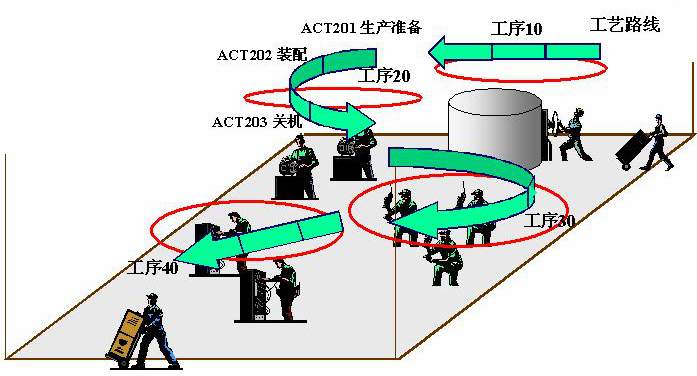
\includegraphics[scale=0.5] {flow1.png}
        \end{center}
    \subsection {工艺路线的定义}

\newcommand{\techflowTab}[1]{
    \begin{tabular}{|c|c|c|c| *9{@{}c@{}|} c|}
        \hline
        \multirow{2}{*}{工序}
            & \multirow{2}{*}{ \shortstack{工序\\名称}}
            & \multicolumn{2}{c|}{工作中心}
            & \multicolumn{3}{c|}{标准时间(小时)}
            & \multirow{2}{*}{ \shortstack{排队\\时间\\(天)}}
            & \multirow{2}{*}{ \shortstack{传送\\时间\\(天)}}
            & \multicolumn{2}{c|}{工人数}
            & \multirow{2}{*}{ \shortstack{外协费\\(元)} }
            & \multirow{2}{*}{工具} \\
                \cline{3-7} \cline{10-11}
        & & 编号 & 名称 & 准备
            & \shortstack{加工\\(工时)}
            & \shortstack{机器\\(台时)} & & & 准备 & 加工 &&\\
        \hline
        #1
        \hline
    \end{tabular}
}

    工艺路线是说明零部件加工或装配过程的文件。在MRP系统中,编制工艺路线是在工艺过程卡的基础上进行的,但又有所不同。前者是指导加工制造的技术文件,后者是计划文件或管理文件。为了使报表比较简练,通常并不详细说明与编制计划没有直接关系的技术要求和方法 (必要时可在注释中说明)。

    工艺路线的典型报表格式如表\ref{tab:techflowReport}所示。

    \begin{table}[bcth]
        \footnotesize
        \caption{工艺路线典型报表格式} \label{tab:techflowReport}

        \vskip 1em
        \begin{tabular}{l c m{10em} l c}
            物料号: & 11100 & & 生效日期: & 20031014 \\
            物料名称:& C & & 失效日期:& 20040430 \\
        \end{tabular}

        \centering
        \techflowTab{
            10&下料&17100&锯床&0.5&0.25&--&1.0&1.0&1&1
               &\multirow{6}{*}{200.00}
               &\multirow{6}{*}{\shortstack{逐个\\工序\\分别\\列出\\菜单}} \\
            20&车削&61214&车床&1.0&1.25&--&1.0&1.0&1&1  &&\\
            30&热处理&06010&电炉&1.2&--& $5.00^*$ &2.0&1.0&2&1  &&\\
            40&磨削&02052&磨床&1.0&2.00&--&3.0&1.0&1&1  &&\\
            50&电镀&90001&(外协)&--&--&--&--&10.0&--&--  &&\\
            60&检验&08015&质检&--&0.10&--&1.0&--&--&1  &&\\
        }
    \end{table}


\subsection {工艺路线的作用}

    工艺路线主要有以下作甩

    \begin{itemize}
        \item 计算加工件的提前期,提供运行 MRP 的计算数据;
        \item 计算占用工作中心的负荷小时,提供运行能力计划的数据;
        \item 计算派工单中每道工序的开始时间和完工时间;
        \item 提供计算加工成本的标准工时数据;
        \item 按工序踉踪在制品,是工序跟踪报告的依据。
    \end{itemize}

\subsection {工艺路线报表}

    工艺路线报表有以下特点

    \begin{enumerate.zh}
        \item 除说明工序顺序、工序名称、工作中心代码及名称外,工艺路线报表还把加工过程和时间定额汇总到一起显示。制定工时定额同编制工艺在同一部门进行。工艺人员掌握时间定额,有助于分析所制订的工艺的经济合理性。

        \item 除列出准备和加工时间外,还列出排队时间和等待/传送时间,也就是加工前后的缓冲时间。

        \item 表上列出的准备和加工的标准时间,是用来计算标准成本用的,考虑了操作工人的人数。在计算计划跨度和能力计划负荷时,要被相应的工人数除,才是真正占用工作中心的时间,再连同传送、排队时间作为编制计划进度的依据。例如,工序 10 的加工标准时间为 0.5,这是计算成本用的数据,即加工一件消耗 0.5 工时,再乘以工时费率。如果计算计划跨度和能力,要被这道工序的加工工人数 2 除,即 0.25 小时,也就是占用工作中心的时间。

        \item 每道工序对应一个工作中心,说明物料的形成同工作中心的关系,也用来说明工作中心负荷是由于加工哪些物料形成的。

        \item 工艺路线表包括了外协工序、外协单位代码和外协费用。外协工序的时间可记入工序的传送时间字段中,表示工件从送出到收回的时间,是固定提前期。

        \item  除了说明基本的工艺路线外,还要说明各种可能替代的工艺路线,便于在调整计划或主要工艺路线上的设备出现故障时替代。当一个零件可以通过多种的工艺路线完成,或有若干替代工艺路线,可对不同工艺路线赋予不同代码。若工艺路线比较定型,使用同一类型工艺路线的零件较多时(如成组加工),但每件的加工时间又不同时,也可对典型的工艺路线编碼。利用软件的复制功能,建立新的工艺路线时只需修改少量数据,简化数据录入。此外,和建立物料清单一样,也要说明工艺路线的生效期和失效期。

       \item 系统在模拟计划时,如需要调整工艺可先对工艺路线的工序变化、时间定额、加工成本进行模拟,然后再做决策。
    \end{enumerate.zh}

\subsection {工艺路线与物料清单结合应用}

    工艺路线有时要结合物料清单来应用。例如,对由企业提供毛坯或原材料委托外协加工的物料。由于原材料作为企业的采购件必须列入产品结构,而外协件作为原材料的母件,不在产品结构的最低层,不能定为采购件,但却要作为采购作业对待。 这时,可用一种变通的办法,把外协件定义为加工件,但其工艺路线只有一道外协工序(这种处理方法还要依软件功能而定)。表 \ref{tab:wanjiaoReport}是电阻件外协弯脚的例子。

    \begin{table}[bcth]
        \footnotesize
        \caption{自购材料外协加工的处理方法} \label{tab:wanjiaoReport}

        \vskip 1em
        \begin{tabular}{l c m{10em} l c}
            物料号: & 47588 & & 生效日期: & 20031014 \\
            物料名称:& R & & 失效日期:& 20040430 \\
        \end{tabular}

        \centering
        \techflowTab{
            10 & 弯脚 & 90003 & (外协) & -- & -- & -- & --
            & 15.0 & -- & -- & 385.00 & \\
        }
    \end{table}

    从逻辑讲,工艺路线中可以把"设计”、"运输” 等非工艺性作业,作为独立需求件性质的一道工序来处理。也可以把供应商或分包商的计划,作为一种特定的工序对待,只计算提前期和总费用。只要符合运算逻辑,根据软件的条件,可以有各种灵活的变通应用。

    总之,可以按照逻辑关系,灵活运用工艺路线的功能。它可以包括任何占用工作中心需要计算时间的工序,也可以是既无工作中心又无费用但要增加时间的 "工序”。

    在机械产品中,往往有两件相关的物料分别加工后,再合在一起加工,然后又分开加工的情况。如箱体和箱盖、连杆体和连杆盖、涡轮副或油泵油偶件等(又称配作件。在采用数控机床加工的情况下,某些配作可以减少)。 这些加工件的工艺路线需特殊处理。不同工序加工批量不同时,如车削与热处理,有时需要把热处理作为单独物料处理,在物料清单上要增加一个层次。

    换句话说,编制物料清单要同工艺路线结合起来考虑,在流程工业中这种特点更为普遍。
 % 工艺路线的定义

\section {质量检验标准}
    \section {什么是质量}

    品管应该完成的所有工作,可以说就是质量管理的中心业务,而其业务又以防止不良的发生为重点,从这个意义上看,关于质量的机能,它有如图\ref{fig:qcMech}所示的业务。

    \begin{figure}[h]
        \centering
        \begin{tikzpicture}[
                fun/.style={
                    draw,
                    inner sep=1em,
                    fill=white,
                    drop shadow,
                    },
                nc/.style={
                    edge from parent/.style={draw=none},
                    level distance=2.2em,
                    font=\itshape,
                    },
                ]
            \node[fun]{品质技能}
            [edge from parent fork down, level distance=6em, sibling distance=8em]
                child{node[fun]{品质检查}
                    child[nc]{ node{(验收机能)} }
                    }
                child{node[fun]{品质管理}
                    child[nc]{ node{(预防机能)} }
                    }
                child{node[fun]{品质保证}
                    child[nc]{ node{(保证机能)} }
                    }
                ;
        \end{tikzpicture}
        \caption{质量管理的品质机能}    \label{fig:qcMech}
    \end{figure}

    质量不是光靠检查就能确保的,要确保质量必须能正确地执行合理的设计、正当的工程管理等品管(预防机能)业务。也就是说,质量保证工作就是调查品管业务是否实行得当,调查设计、制造、销售等各部门是否确保了目标的质量,并将此结果向经营者报告。

\section {质量保证活动范围}

  质量保证活动不只是各部门在各阶段的业务执行(部门内的活动)与管理动,它还包含部门与部门之间的活动及其管理(机能管理)。更重要的是,不只是明确活动的管理方法,并要求确实执行,同时还必须对质量的管理,即质计划、质量传达、质量确认等采取相同措施。以下以项目形式列举了质量保证活动的范围:

    \begin{enumerate}
        \item 质量的设计,新品种、新制品质量的设定,规格的设定、修正与废除。

        \item 材料的购人与保管: 材料管理、库存管理。

        \item 标准化。

        \item 工程的解析与管理。

        \item 检查及不合格产品的处理。

        \item 客诉处理、质量稽查。

        \item 例设备管理:设备的建设、预防保养、计测管理。

        \item 人事劳务管埋: 适当正确的职务分配、教育训练。

        \item  外包、转包管理。

        \item 技术开发: 新制品的开发、研究管理、技术管理。

        \item 诊断与稽查: 质量管理实施状况的诊断、品管关系业务稽查。
    \end{enumerate}

\section {质量保证体系设立}

    在设立质量保证体系时,应注意以下几点

    \begin{enumerate}
        \item 回馈的方法必须明确。

        \item 体系图的纵轴表示开发的阶段,横轴表示职别,此职别的负责人必须明确有关内容。

        \item 对体系运作的手段,用具(表单类)及运作规则必须予以确定。

        \item 决定是否可以向下一阶段运作的评价项目与评价方法必须明确。

        \item 必须由体系运作所带来的经验来修正体系。
    \end{enumerate}

\section {质量组织计划}

    在质量管理的推进计划中,最重要的是“组织计划”。

    \begin{enumerate}
        \item 组织计划应害虑的事顶:

            在组织计划中要考虑以下事项

            \begin{enumerate}
                \item 质量管理的组织,并不是指成立质量管理部或品管科,而必须是:
                    \begin{itemize}
                        \item 让所有相关人员都知道有关产品质量情报的信息系统。

                        \item 在质量管理活动中,动员企业内所有的部门,所有阶层人员的方法。
                    \end{itemize}

                \item 是否有因人而设立组织,因组织而设立工作的倾向?

                \item 是否充分进行授权? 其授权工作不能只是口头说说,必须以文件加以明确。

                \item 组织之间的结合是否完全,品管活动中动员企业所有部门,所有阶层的方法是否确立? 从品管业务角度来看 横向的联系是否充分?

                \item 变更组织时的步骤是否明确?

             \end{enumerate}
        \item 组织计划的原则

        如前所述,组织化并不仅仅是将业务细分,成立各种职能部门,为了达到质量目标,还必须使其分担质量管理的责任与权限。 因此,组织必须满足以下原则:

            \begin{enumerate}
                \item 组织的上级与下级之间必须有明确的权限关系。这里所说的权限是指要求其他人活动的正常权利。

                \item 组织中的每一个人应固定地向生产线的某一主管报告,并且要明白自己必须向谁或谁向自己报告。

                \item 经营者、管理者的责任与权限必须以文件形式明确限定。

                \item 权责要相符。

                \item 必须尽量缩减管理层次。

                \item 管理者必须致力于标准化,防止例外或异常情况的发生。

                \item 每一位管理者能够使其协力帮忙的职位数(也即管理幅度)有一定限制。一般情况下,高层的管理幅度为3\~6人,中层为5\~9人,低层为7\~15人。

                \item 组织应具有弹性,必须能顺应形势的变化而有所改变。

                \item 制度必须简明,即阶层的数目不要太多。
            \end{enumerate}

        在这种情形下,下层职位的人只要向自己生产线的主管报告,接受其指示就行了。职位间指挥命令的混乱,只要能明确职位所应管理的项目,即能化解。
    \end{enumerate}
 % 什么是质量
    \section {制定检验标准}

    检验标准应以文件的形式固定下来,用以规定及指明检验作业的执行方法,以便于在繁杂的检验作业中,处理各种疏漏与不足。

    \begin{enumerate}

    \item 明确制定检验标准的目的

        使检验人员有所依据,了解如何进行检验工作,以确保产品质量。

    \item 巳列明检验标准内容

        \begin{enumerate}
            \item 适用范围 。列明适用于何种进料(含加工品) 或成品的检验。

            \item 检验项目。将实行检验时应检验的项目一一列出。

            \item 质量基准。明确规定各检验项目的质量基准,以此作为检验时判定的依据。如无法以文字述明,则用限度样本来表示。

            \item 检验方法。说明在检验各种项目时,使用何种检验仪器、量规、或是以感官检查(例如目视)的方式来检验; 如某些检验项目须委托其他机构代为检验,也应注明。

            \item 抽样计划。采用何种抽样计划表(例如,计数值用MIL-SID-105D,计量值用MIL-STD-414)。

            \item 取样方法。抽取样本,必须由群体批中无偏倚地随机抽取,可利用乱数表来取样,但群体批各制品无法编号时,则取样时必须从群体批的任何部位平均抽取样本。

            \item 群体批经过检验后的处置。
                \begin{itemize}
                    \item 属进料(含加工品)者,依进料检验规定的有关要点办理(如是台格批,则通知仓储人员办理人库手续,如是不合格批,则将检验情况通知采购单位,由其根据实际情况决定是否需要特采)。

                    \item 属成品者,依照成品质量管理作业办法有关要点办理(合格批人库或出旨,不合格批则退回生产单位检修)。

                \end{itemize}
            \item 其他应注意的事项。

                \begin{itemize}
                    \item 如按特定的顺序来检验各检验项目时,必须将检验顺序列明。

                    \item 必要时,可将制品的蓝图或略图置于检验标准中。

                    \item 详细记录检验情况。

                    \item 检验时在样本中发现的不良品,以及在群体批次中偶然发现的不良品,应与良品交换。

                    \item 其他。
                \end{itemize}

            \end{enumerate}

    \item 有关检验标准的制定与修正

        由工程单位、质量管理单位制定。

    \end{enumerate}

\section {制定检验作业指导书}

    \begin{enumerate}
        \item 检验作业生旨导书的适用范围

        以下情况应编制检验作业指导书:

            \begin{enumerate}
                \item 对工序质量控制计划中设置丁工序质量控制点的检验。

                \item 对关键和重要零件的检验。

                \item 新产品特有的检验活动。

            \end{enumerate}
        \item 检验作业指寻书的内容

            \begin{enumerate}
                \item 检验对象。主要为受检物的名称、图号,必要时还须说明其在检验流呈图上的位置(编号)。

                \item 质量特性。规定的检验项目,须鉴别的质量特性、规范要求,质量特性的重要性级别,所涉及的质量缺陷严重性级别。

                \item 检验方法。检验基准,检测程序与方法,检测中的有关计算方法,检测频次,抽样检验的有关规定及数数据。

                \item 检测手段。检测使用的工具,设备(装备)及计量器具,这些器物应处的状态,使用中必须指明的注意事项。

                \item 检验判断。正确指明对判断标准的理解,判断比较的方法、判定的原则注意事项,不合格品的处理程序和权限

                \item 记录和报告。指明需要记录的事项与方法和表格,规定要求报告的内容、方式、程序与时间。

                \item 其他。对于复杂的检验项目,检验作业指导书应给出必要的示意图表并提供有关的说明资料。

            \end{enumerate}

        \item 检验作业指导书的格式

        作业指导书没有固定的格式,作业指导书常采用表格或流程图形式,也可采用图文并茂的形式。

    \end{enumerate}

 % 制定检验标准

\practices

\subsection{工艺管理}
\opset{工艺管理}{
    \item \ops{新建工艺}{
        \item  点击\button{新建}按钮,弹出新建工艺对话框
            \screenshot{1.png}
        \item  输入工艺\textbox{名称}
        \item  输入工艺\textbox{描述}
        \item  点击\button{保存}完成新增工艺
    }
    \item \ops{查看工艺}{
        \item 选择需要查看的工艺
        \item  点击工具栏上的\button{查看}按钮,查看工艺详细信息
    }
    \item \ops{修改工艺}{
        \item  选择需要修改的工艺,点击\button{修改}按钮,弹出修改对话框
            \screenshot{2.png}
        \item  修改相应的工艺\textbox{名称}
        \item  修改相应的工艺\textbox{描述}
        \item  点击\button{保存}按钮完成修改
    }
    \item \ops{删除工艺}{
        \item  选择需要删除的工艺
        \item  点击\button{删除}按钮,弹出确认删除对话框
            \screenshot{3.png}
        \item  点击确定完成删除
    }
}

\subsection{BOM管理}
    \opset{BOM管理}{
    \item \ops{新建BOM物料清单}{
        \item  点击工具栏上的\button{新建}按钮,弹出新建BOM物料清单对话框
            \screenshot{4.png}
        \item  在\button{基本信息}标签下选择\button{物料}
        \item  输入\textbox{生效}
        \item  输入\textbox{失效}日期
        \item  输入\textbox{工资}
        \item  输入\textbox{电费}
        \item  输入\textbox{设备费}
        \item  输入\textbox{其他费用}
        \item  在\button{BOM明细}标签下,点击\button{添加}按钮,弹出添加明细对话框
            \screenshot{5.png}
        \item  \button{选择成品}或者\button{半成品}作为清单项目之一
        \item  勾选\button{是否有效}
        \item  选择BOM清单项目的\button{生效},\button{失效日期}
        \item  输入\textbox{数量}
        \item  输入\textbox{描述}
        \item  点击\button{确定}按钮,完成一个清单项目的添加
        \item  点击\button{保存}按钮,完成新建BOM物料清单
    }
    \item \ops{查看物料详细}{
        \item  选择物料清单
        \item  点击工具栏上的\button{查看}按钮,查看BOM物料清单详细
    }
    \item \ops{修改物料清单}{
        \item 选择物料清单,点击工具栏上的\button{修改}按钮,弹出修改BOM清单对话框
            \ul {
            \item  修改BOM物料清单的\textbox{基本信息}
            \item  修改BOM清单\textbox{明细项目}
            \item  点击\button{保存}按钮,完成BOM物料清单的修改
            }
    }
    \item \ops{工艺设置}{
        \item  选择BOM物料清单,点击工具栏上的\button{BOM树}按钮,弹出工艺设置对话框
            \screenshot{6.png}
        \item  点击\button{设置}按钮,弹出工艺流程设置对话框
            \screenshot{7.png}
        \item  点击\button{添加}按钮,弹出工艺明细对话框
            \screenshot{8.png}
        \item  在\textbox{基本信息}标签下,输入\textbox{工艺基本信息}
            \screenshot{9.png}
        \item  在\button{消耗材料}标签下,点击\button{添加}按钮,弹出工艺消耗材料对话框
        \item  选择\button{消耗材料},输入\item  输入{数量}
        \item  点击\button{确定},添加一种消耗材料
            \screenshot{10.png}
        \item  在\button{质检标准值}标签下,点击\button{添加}按钮,弹出添加质检标准对话框
        \item  输入\textbox{质检内容}
        \item  输入\textbox{标准值}
        \item  输入\textbox{标准描述}
        \item  点击\button{确定},添加一项质检标准
        \item  点击工艺明细对话框下的\button{确定}按钮,完成工艺项目明细设置
        \item  点击\button{保存}按钮,保存工艺设置
        }
    }
